\section{Фильтрация изображений с периодичностью}

Для того, чтобы убрать периодичные части изображения, воспользуемся двумерным преобразованием Фурье. 

Исходное изображение представлено на рисунке \ref{img:src}

\begin{figure}[ht!]
    \centering
    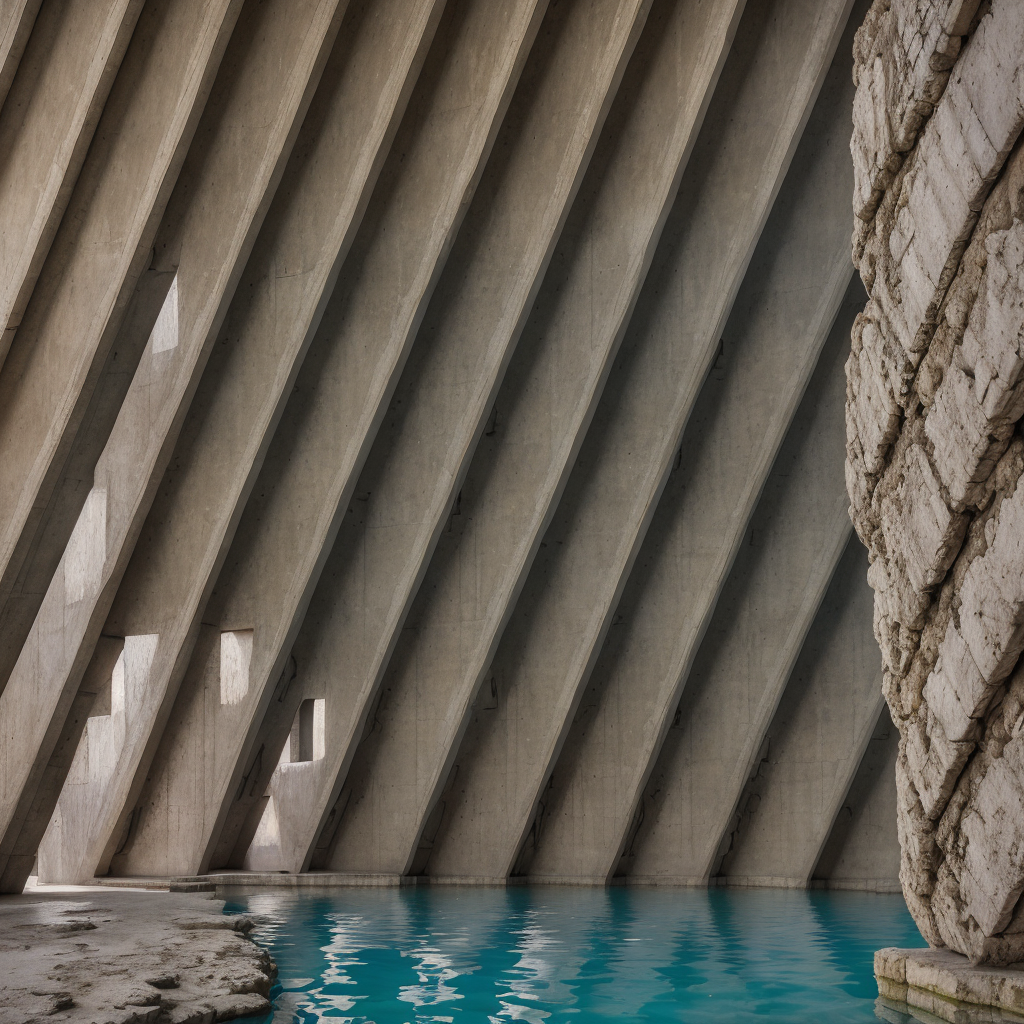
\includegraphics[width=\textwidth]{8.png}
    \caption{Исходное изображение}
    \label{img:src}
\end{figure}

Для начала найдем двумерное преобразование Фурье исходного изображения. Логарифм модуля получившегося результата представлен на рисунке \ref{img:src_fft} 

\begin{figure}[ht!]
    \centering
    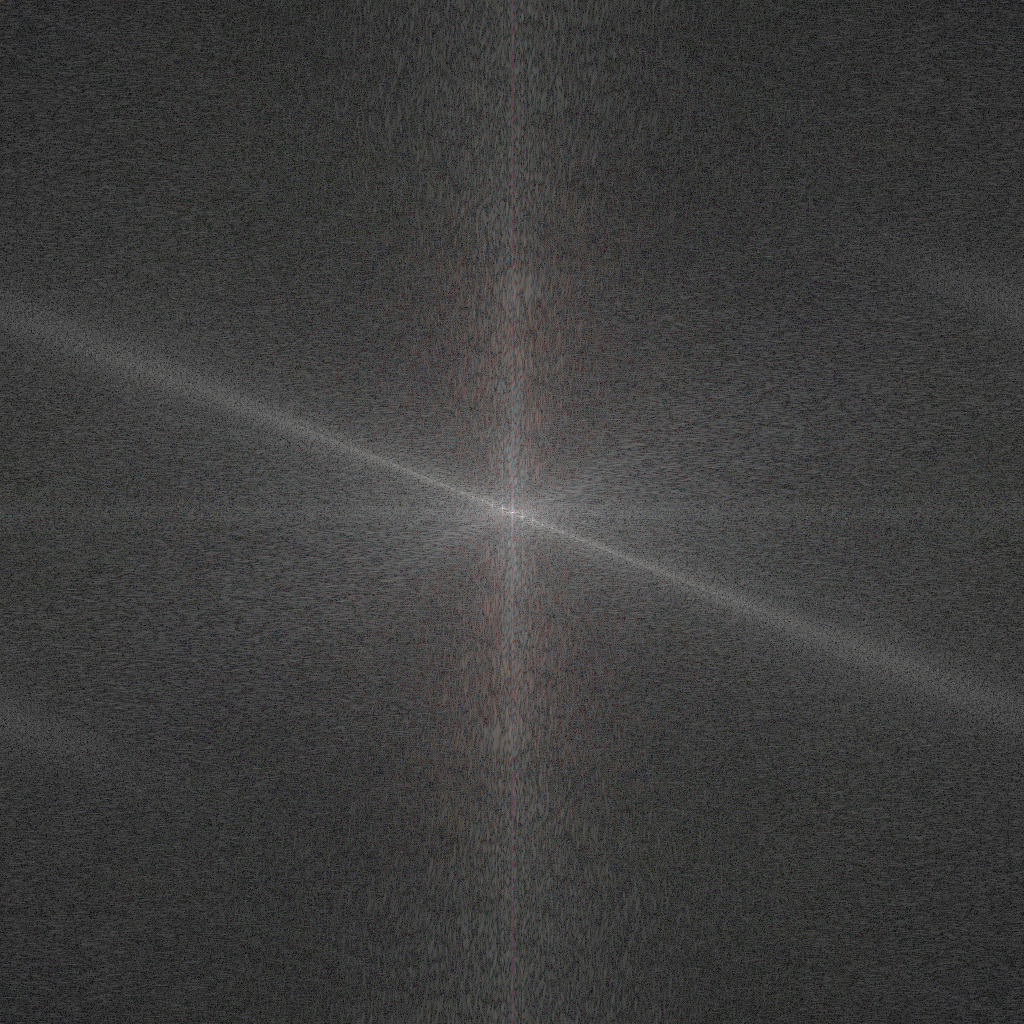
\includegraphics[width=\textwidth]{abs_fourier_log.png}
    \caption{Двумерное преобразование Фурье исходного изображения}
    \label{img:src_fft}
\end{figure}

Видим, что на изображении присутствуют точки, которые соответствуют периодическому шуму, который есть на изображении. 
Для того, чтобы избавиться от периодичности на изображении избавимся от этих пиков на изображении его образа. 

После изменения картинки образа воспользуемся Photoshop. Полученный результат представлен на рисунке \ref{img:fixed}.

\begin{figure}[ht!]
    \centering
    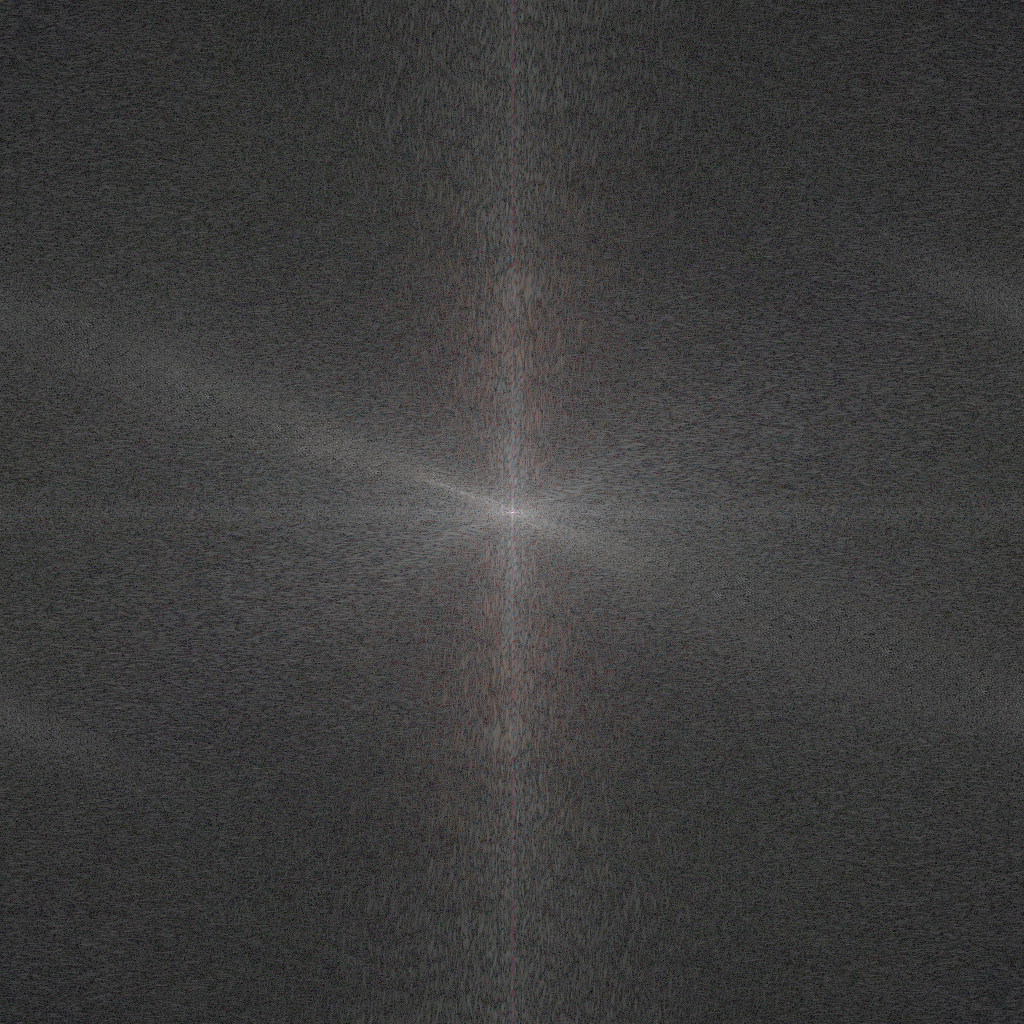
\includegraphics[width=\textwidth]{fixed.png}
    \caption{Исправленный образ}
    \label{img:fixed}
\end{figure}

Теперь воспользуемся обратным двумерным преобразованием для получения изображения обратно. Полученный результат представлен на рисунке \ref{img:restored}. 

\begin{figure}[ht!]
    \centering
    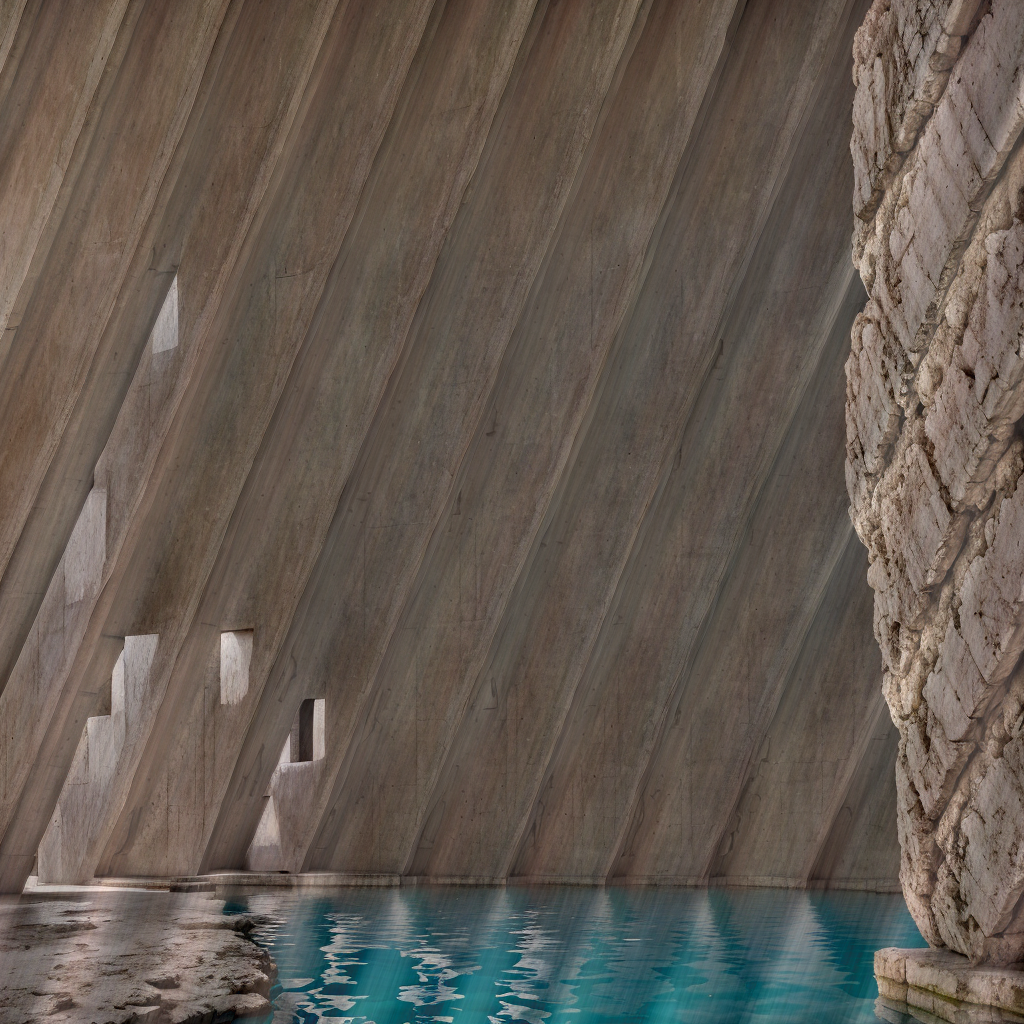
\includegraphics[width=\textwidth]{restored.png}
    \caption{Восстановленное изображение}
    \label{img:restored}
\end{figure}

Видим, что периодичность на изображении стала весьма меньше, чем была изначально.

Сравним исходное изображение и восстановленное. Результат представлен на рисунке \ref{img:compare}.

\begin{figure}[ht!]
    \centering
    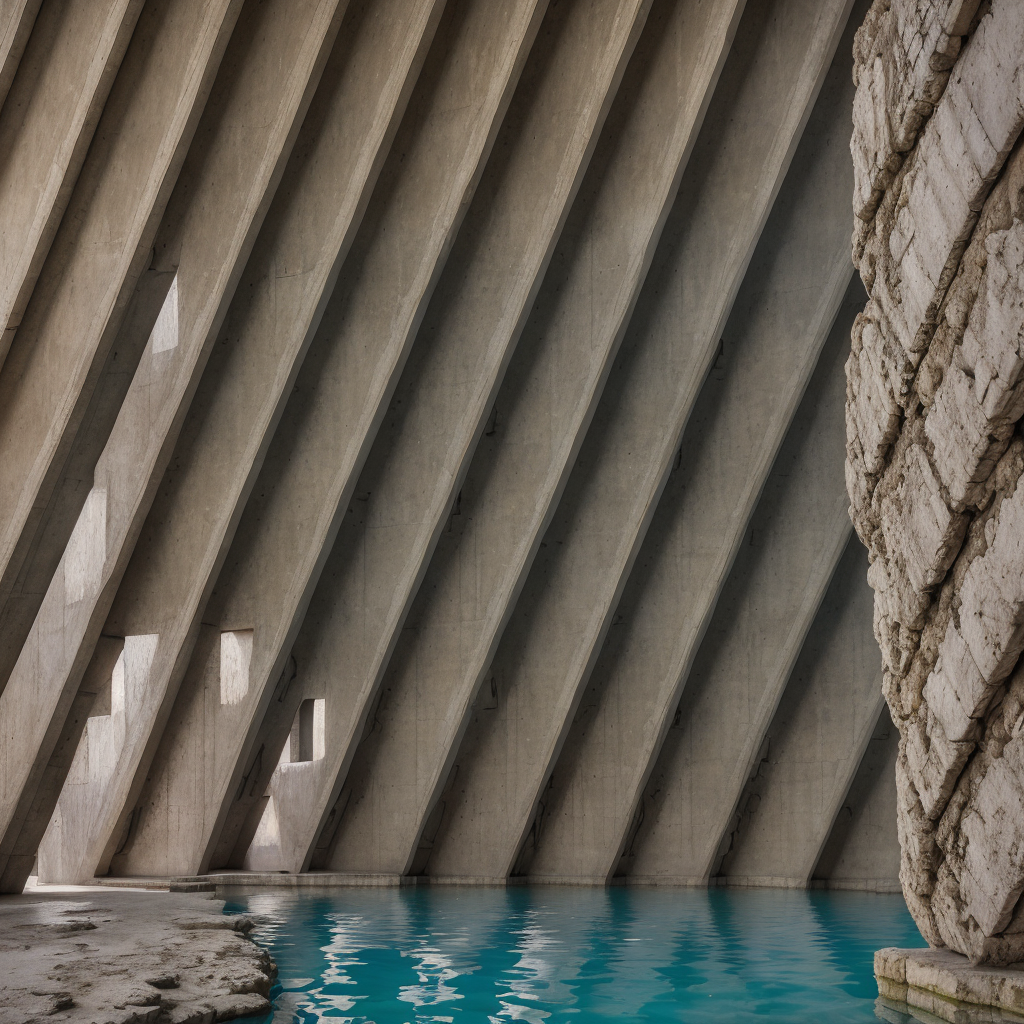
\includegraphics[width=0.49\textwidth]{8.png}
    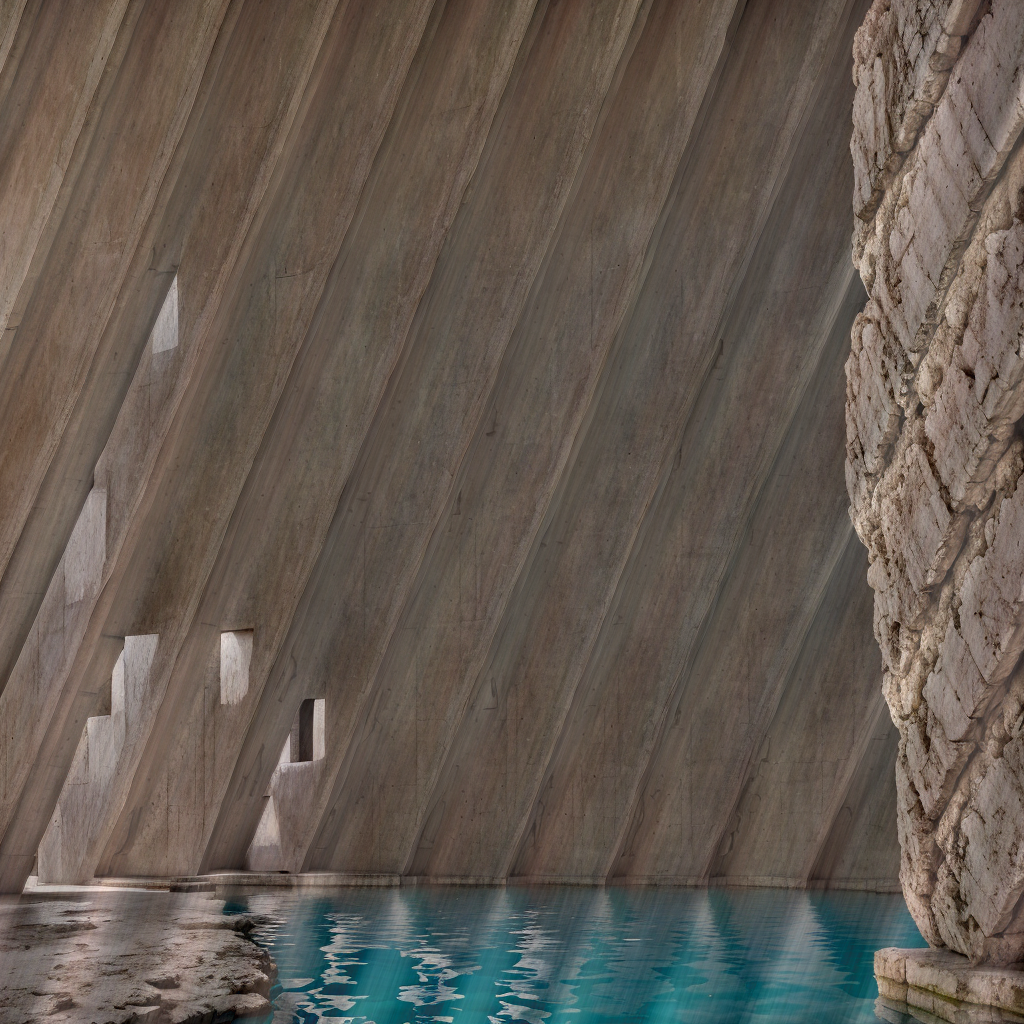
\includegraphics[width=0.49\textwidth]{restored.png}
    \caption{Сравнение исходного и восстановленного изображения}
    \label{img:compare}
\end{figure}

Кроме избавления от периодичности, на изображении также уменьшилась яркость и изменились цвета. 
Это может быть связано с тем, что при изменении образа в Photoshop были затронуты части, которые не были периодичными, но при этом были важными для изображения.


\FloatBarrier
\section{Размытие изображений}

Исходное изображение представлено на рисунке \ref{img:src2}

\begin{figure}[ht!]
    \centering
    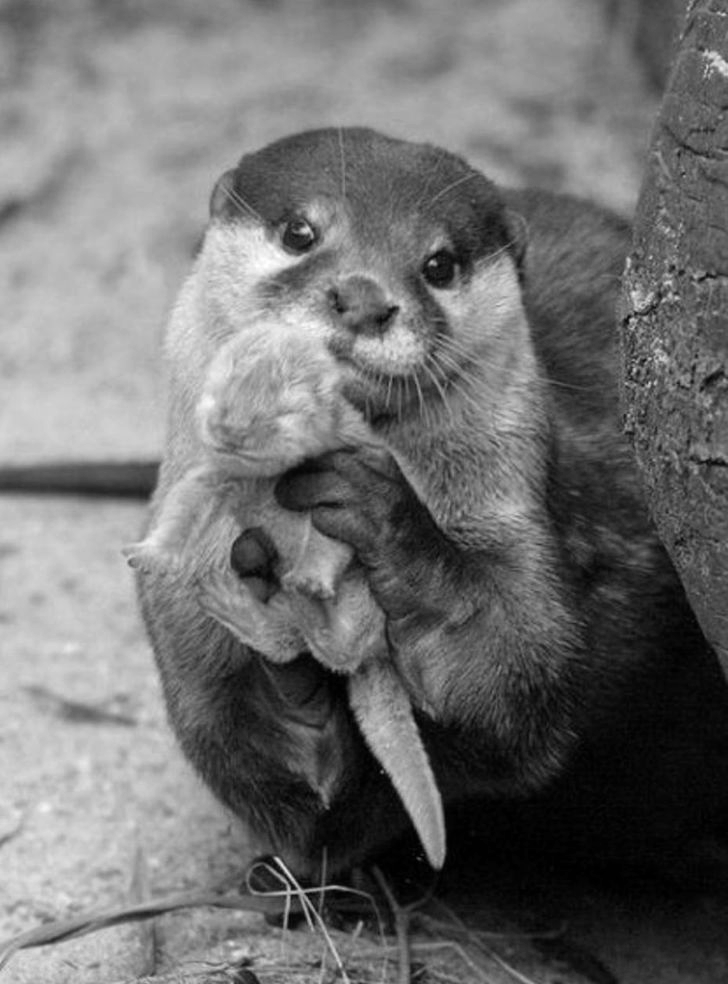
\includegraphics[width=0.5\textwidth]{bw.png}
    \caption{Исходное изображение}
    \label{img:src2}
\end{figure}

Для начала применим к изображению блочное размытие. Результат представлен на рисунке \ref{img:block}

\begin{figure}[ht!]
    \centering
    \begin{subfigure}[b]{0.5\linewidth}
        \centering
        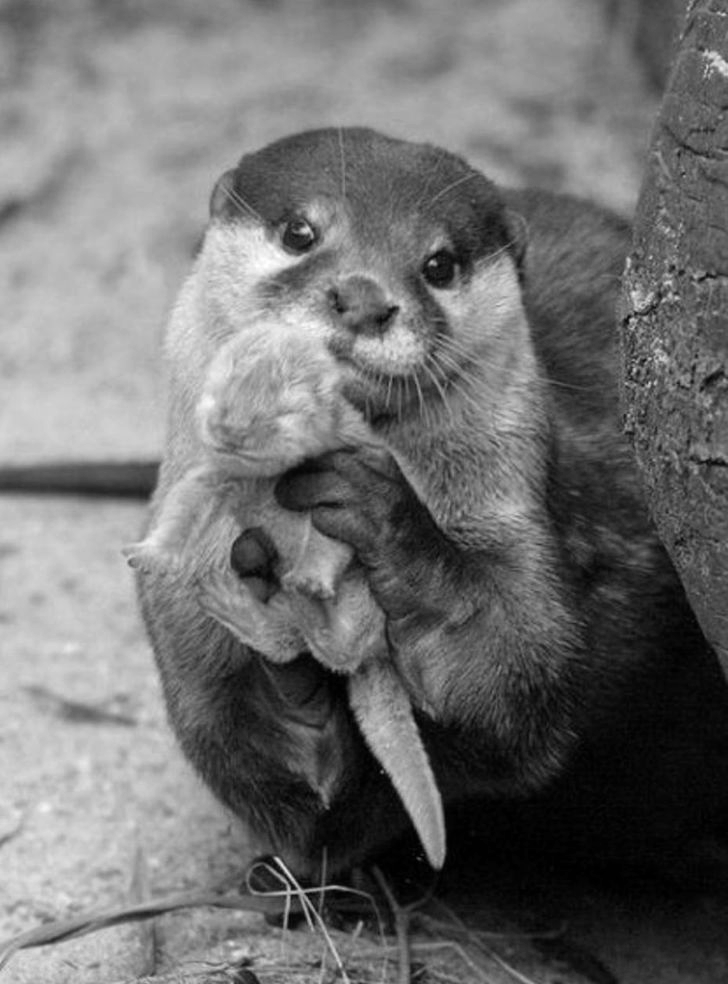
\includegraphics[width=0.95\linewidth]{bw.png}
        \caption{Исходное изображение}
    \end{subfigure}%%
    \begin{subfigure}[b]{0.5\linewidth}
        \centering
        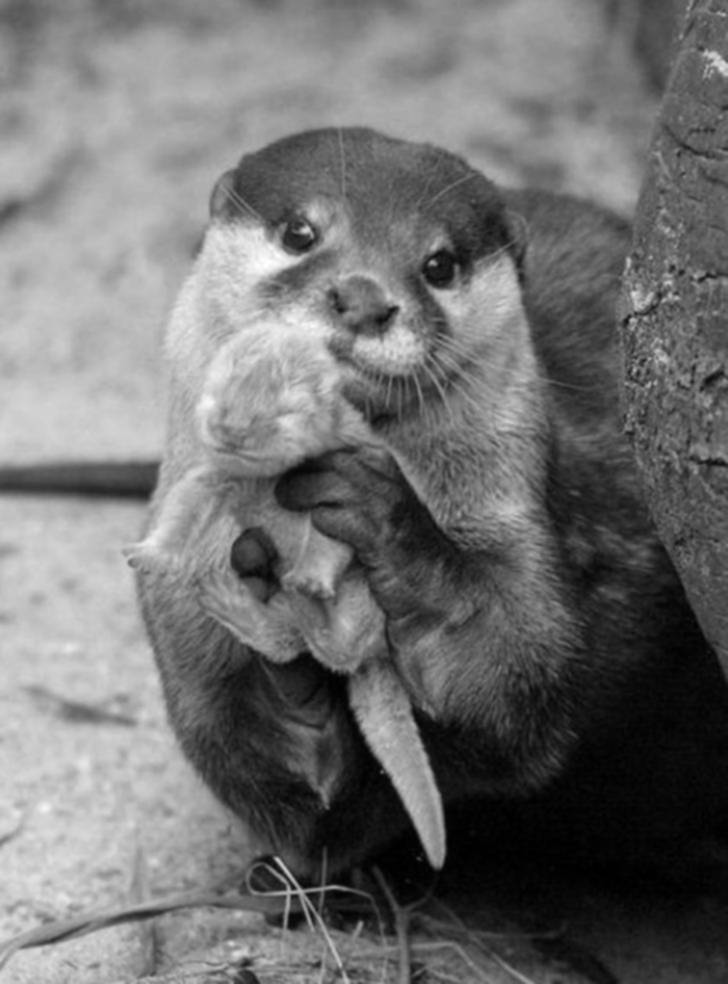
\includegraphics[width=0.95\linewidth]{block_3.png}
        \caption{Блочное размытие, ядро 3x3}
    \end{subfigure}
    \begin{subfigure}[b]{0.5\linewidth}
        \centering
        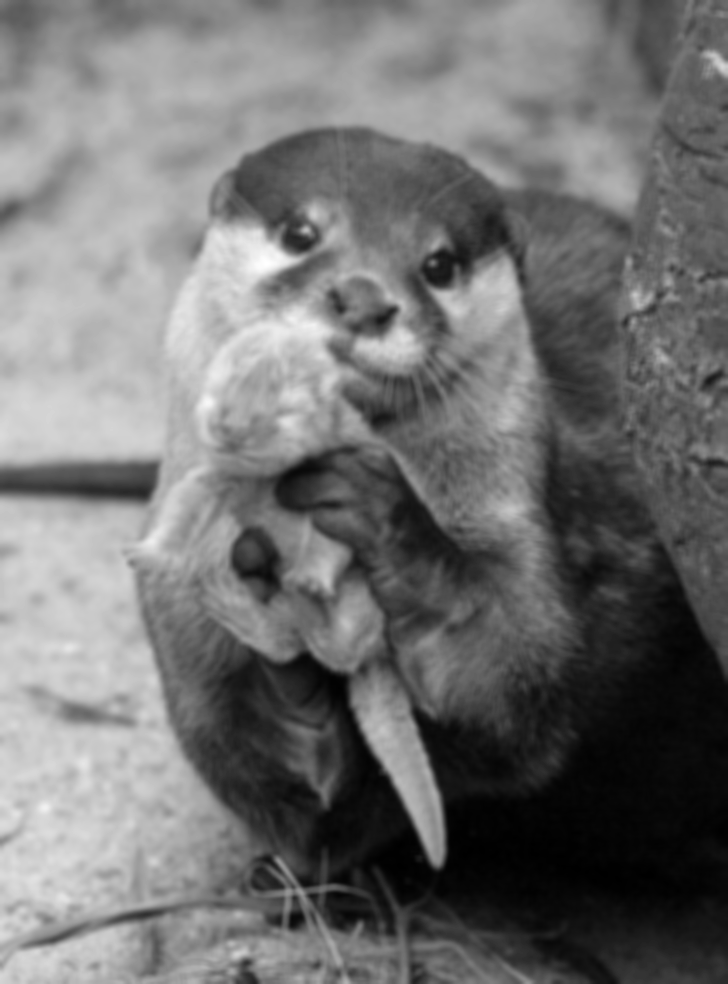
\includegraphics[width=0.95\linewidth]{block_7.png}
        \caption{Блочное размытие, ядро 7x7}
    \end{subfigure}%%
    \begin{subfigure}[b]{0.5\linewidth}
        \centering
        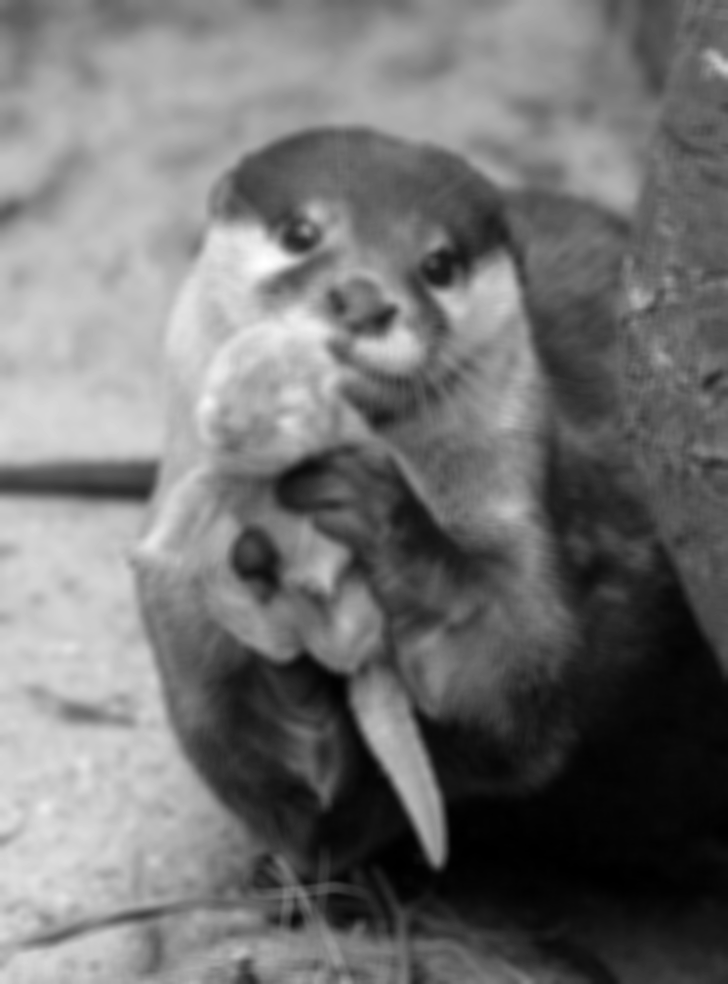
\includegraphics[width=0.95\linewidth]{block_11.png}
        \caption{Блочное размытие, ядро 11x11}
    \end{subfigure}
    \caption{Блочное размытие}
    \label{img:block}
\end{figure}

Теперь применим к изображению размытие Гаусса. Результат представлен на рисунке \ref{img:gauss}

\begin{figure}[ht!]
    \centering
    \begin{subfigure}[b]{0.5\linewidth}
        \centering
        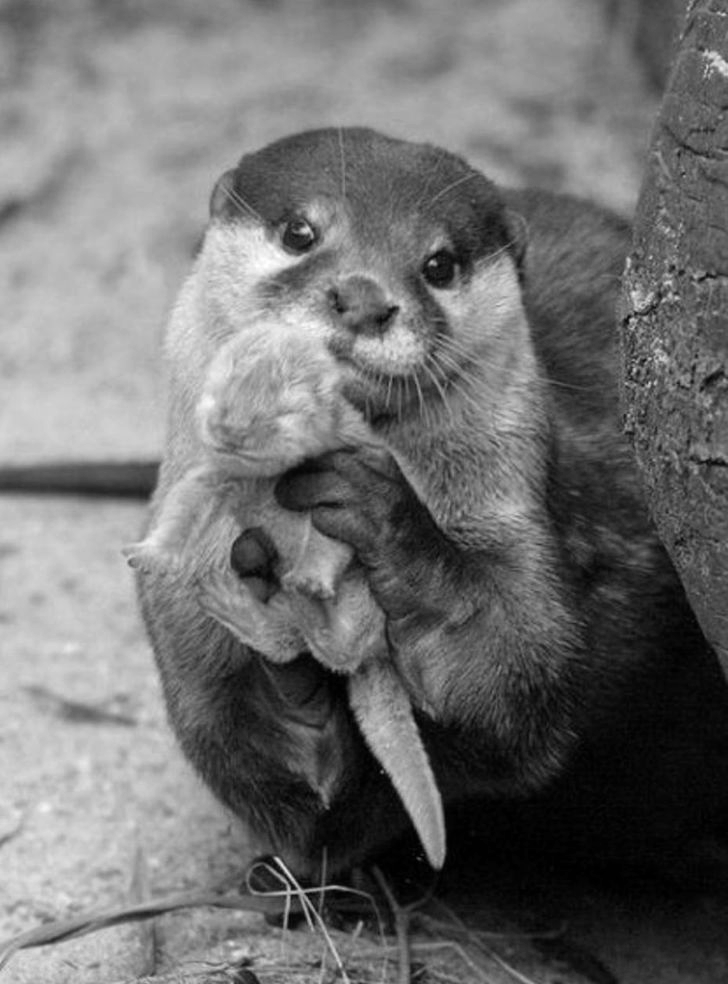
\includegraphics[width=0.95\linewidth]{bw.png}
        \caption{Исходное изображение}
    \end{subfigure}%%
    \begin{subfigure}[b]{0.5\linewidth}
        \centering
        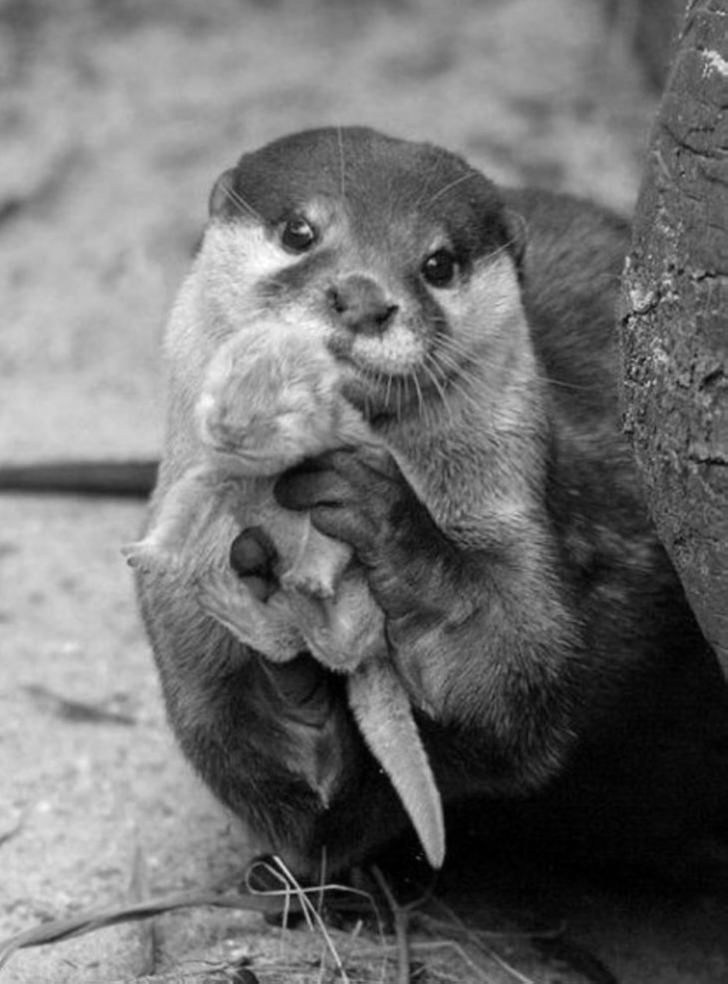
\includegraphics[width=0.95\linewidth]{gaussian_3.png}
        \caption{Размытие Гаусса, ядро 3x3}
    \end{subfigure}

    \begin{subfigure}[b]{0.5\linewidth}
        \centering
        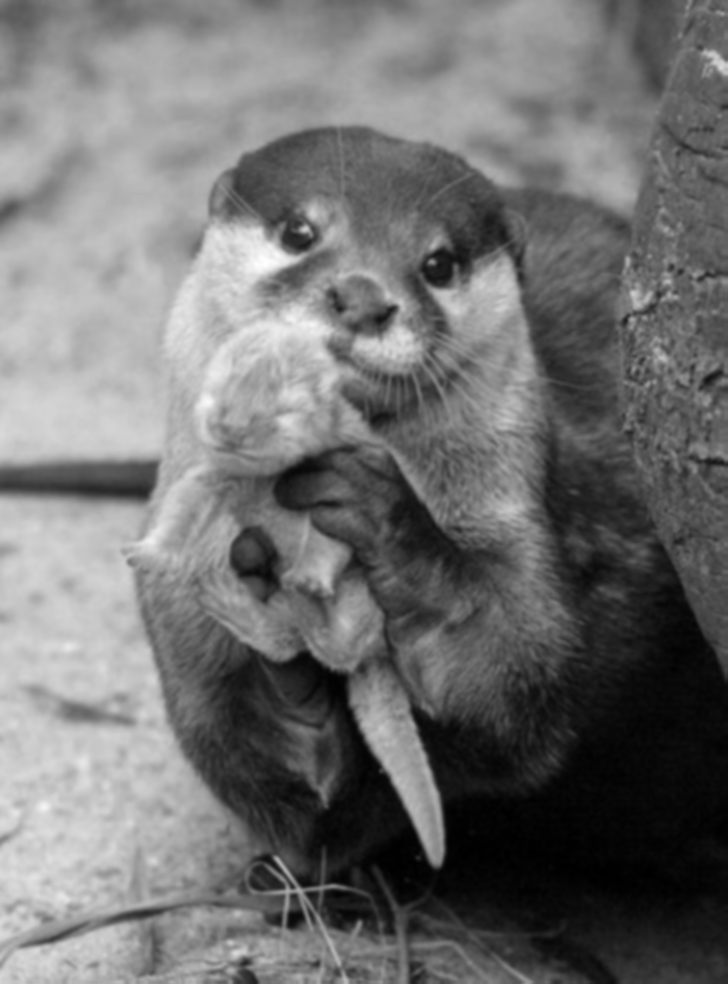
\includegraphics[width=0.95\linewidth]{gaussian_7.png}
        \caption{Размытие Гаусса, ядро 7x7}
    \end{subfigure}%%
    \begin{subfigure}[b]{0.5\linewidth}
        \centering
        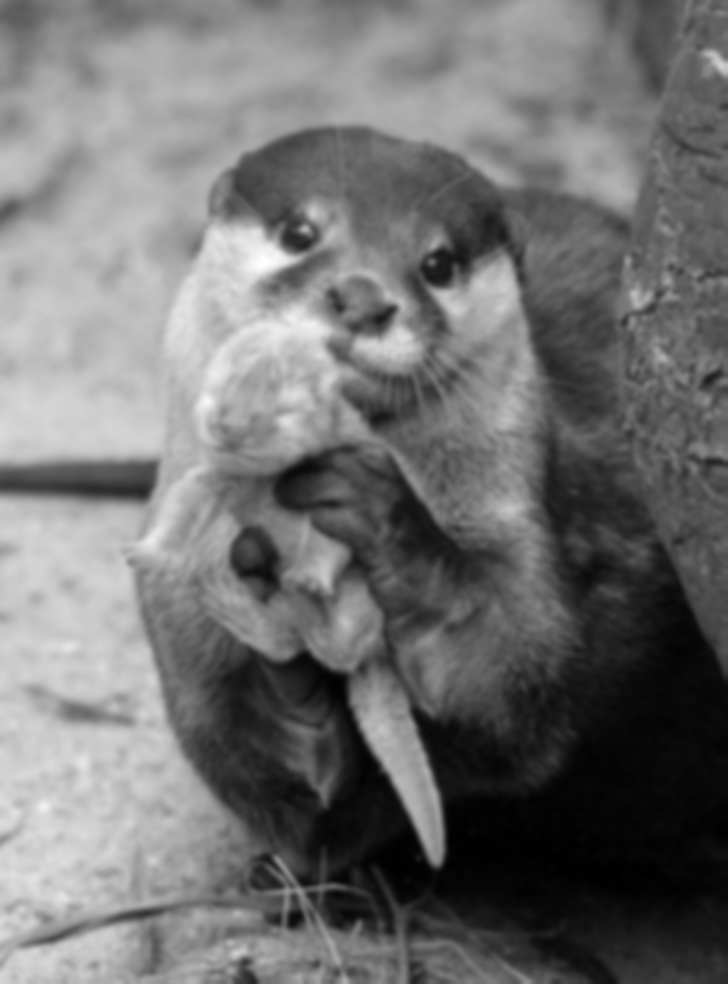
\includegraphics[width=0.95\linewidth]{gaussian_11.png}
        \caption{Размытие Гаусса, ядро 11x11}
    \end{subfigure}
    \caption{Размытие Гаусса}
    \label{img:gauss}
\end{figure}

Как видно из рисунков \ref{img:block} и \ref{img:gauss}, чем больше размер ядра, тем сильнее размытие, что логично.

Теперь применим теорему о свертке для размытия изображения.
\begin{equation}
    X \times Y = \hat{X} \cdot \hat{Y}
\end{equation}

Образ изображения уже был найден в предыдущем пункте. Теперь найдем образ ядра. Для этого дополним 
ядро нулями до размера изображения и найдем его образ. 

Перемножив образ изображения и образ ядра, найдем обратное преобразование Фурье и получим размытое изображение. Результаты представлены на рисунке \ref{img:block2} и \ref{img:gauss2}. 

\begin{figure}[ht!]
    \centering
    \begin{subfigure}[b]{0.5\linewidth}
        \centering
        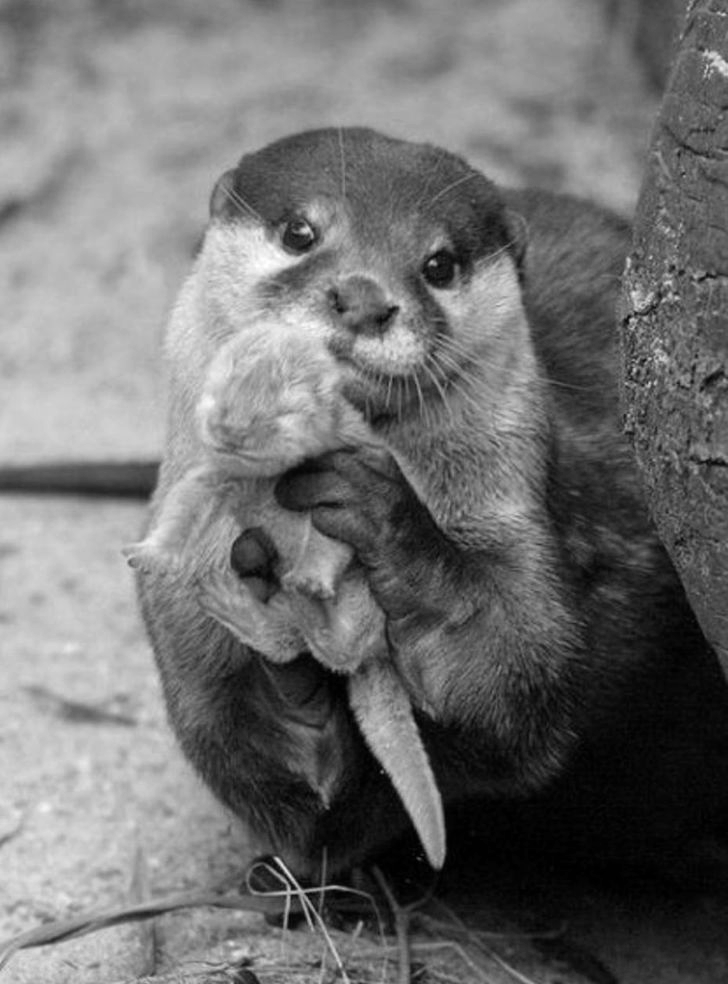
\includegraphics[width=0.95\linewidth]{bw.png}
        \caption{Исходное изображение}
    \end{subfigure}%%
    \begin{subfigure}[b]{0.5\linewidth}
        \centering
        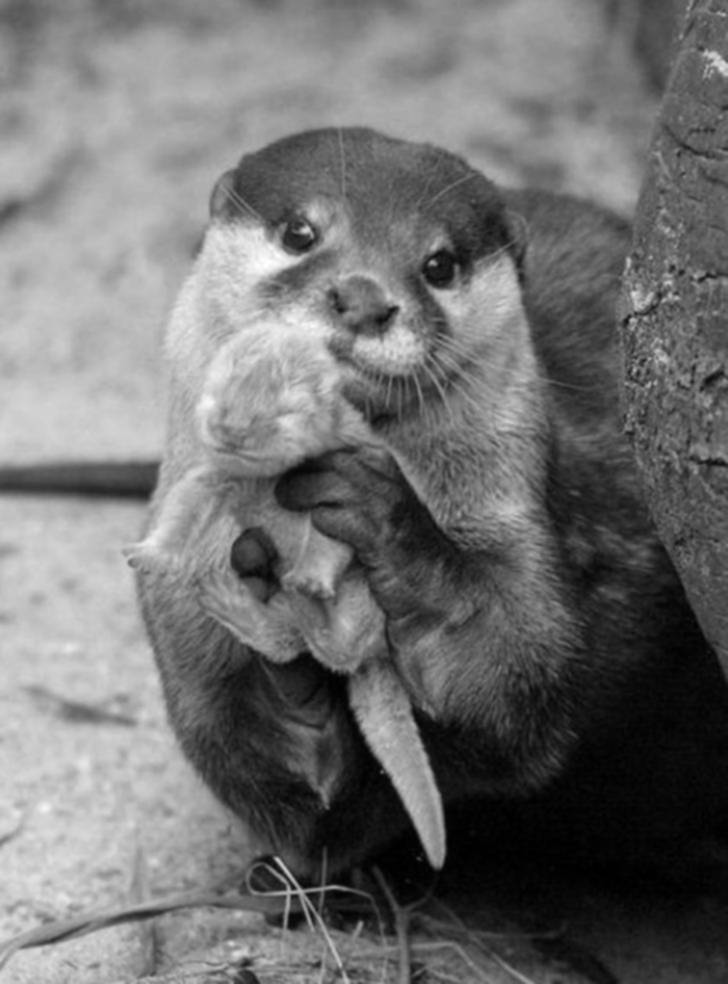
\includegraphics[width=0.95\linewidth]{block_3.png}
        \caption{Блочное размытие, ядро 3x3}
    \end{subfigure}
    \begin{subfigure}[b]{0.5\linewidth}
        \centering
        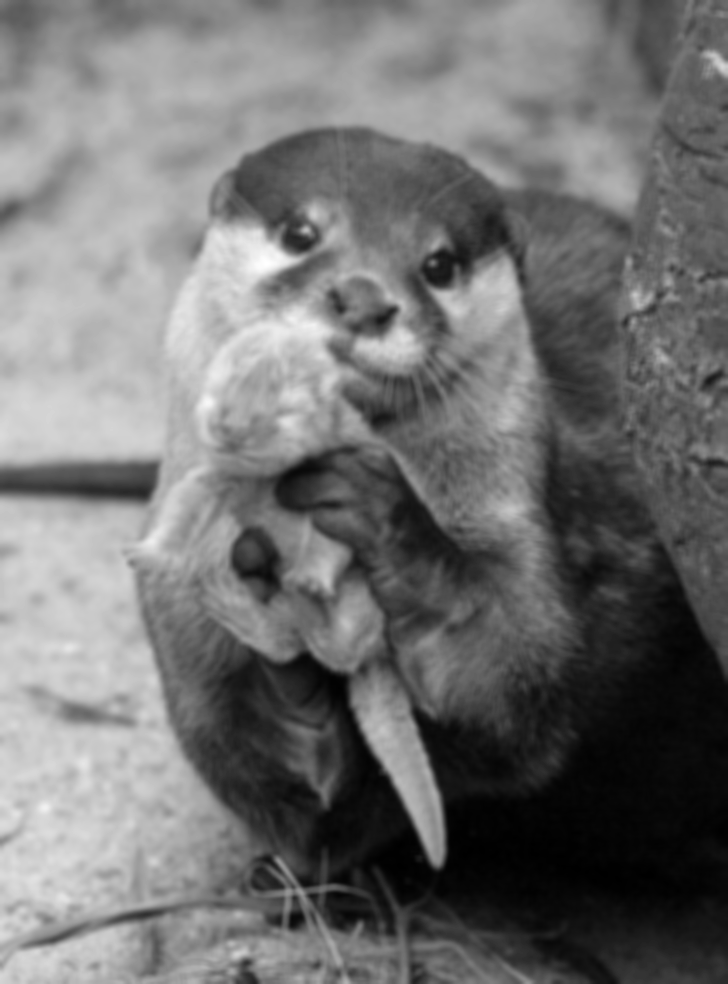
\includegraphics[width=0.95\linewidth]{block_7.png}
        \caption{Блочное размытие, ядро 7x7}
    \end{subfigure}%%
    \begin{subfigure}[b]{0.5\linewidth}
        \centering
        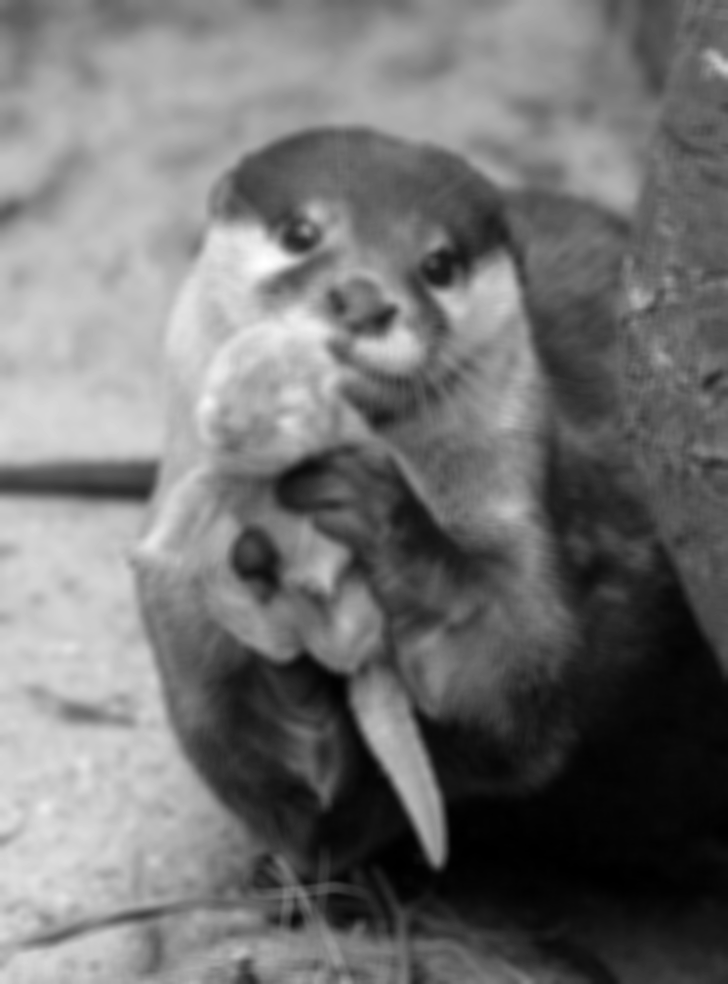
\includegraphics[width=0.95\linewidth]{block_11.png}
        \caption{Блочное размытие, ядро 11x11}
    \end{subfigure}
    \caption{Блочное размытие (через теорему о свертке)}
    \label{img:block2}
\end{figure}

\begin{figure}[ht!]
    \centering
    \begin{subfigure}[b]{0.5\linewidth}
        \centering
        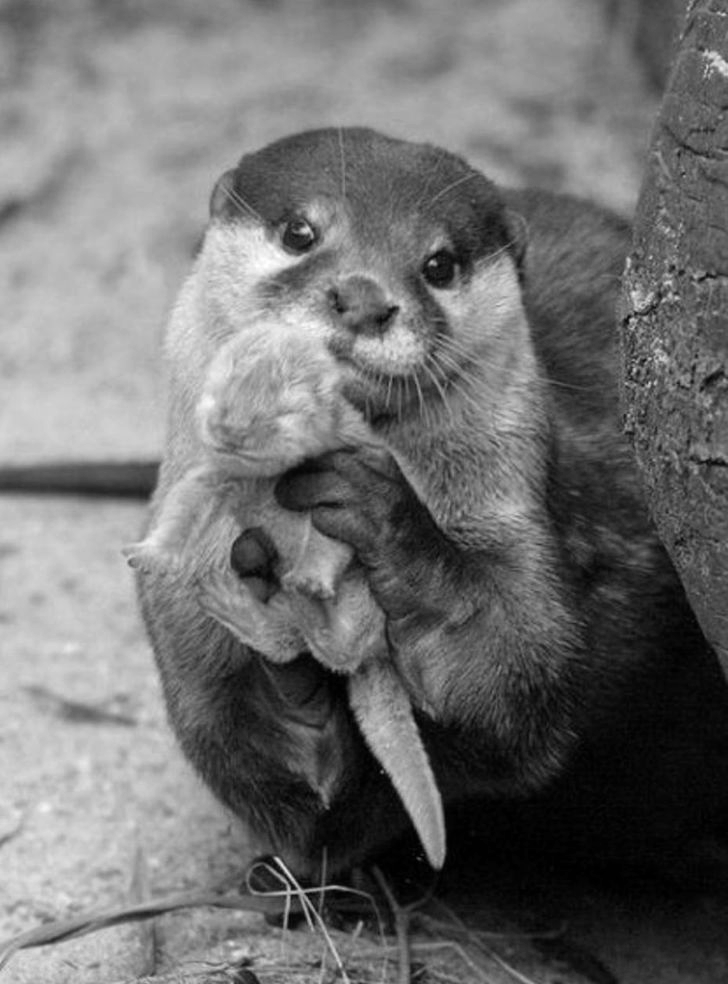
\includegraphics[width=0.95\linewidth]{bw.png}
        \caption{Исходное изображение}
    \end{subfigure}%%
    \begin{subfigure}[b]{0.5\linewidth}
        \centering
        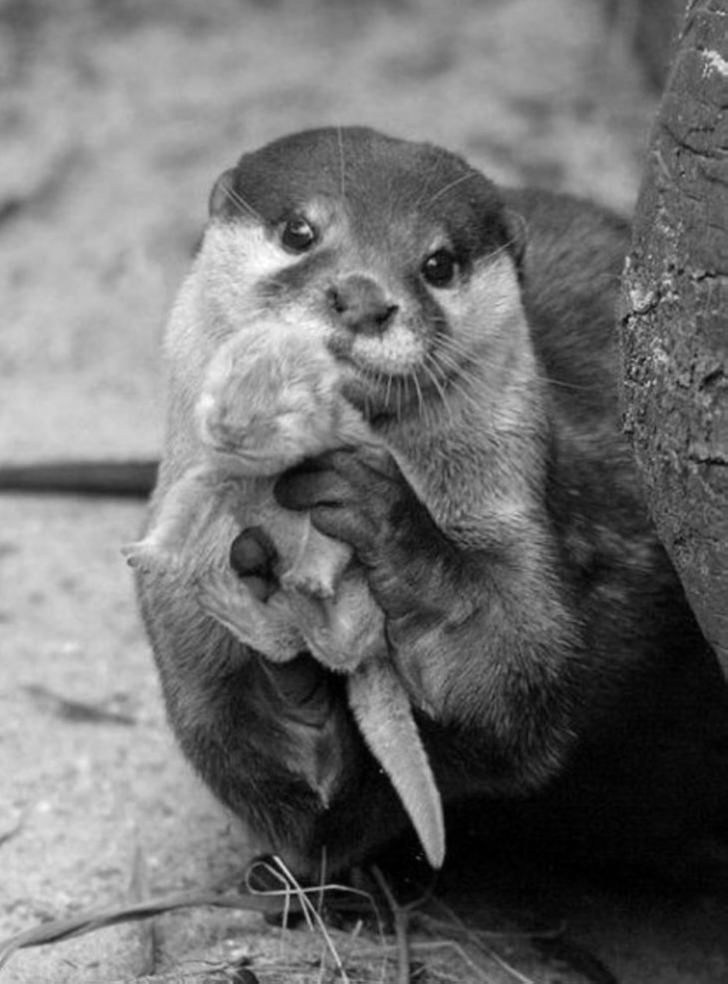
\includegraphics[width=0.95\linewidth]{gaussian_3.png}
        \caption{Размытие Гаусса, ядро 3x3}
    \end{subfigure}

    \begin{subfigure}[b]{0.5\linewidth}
        \centering
        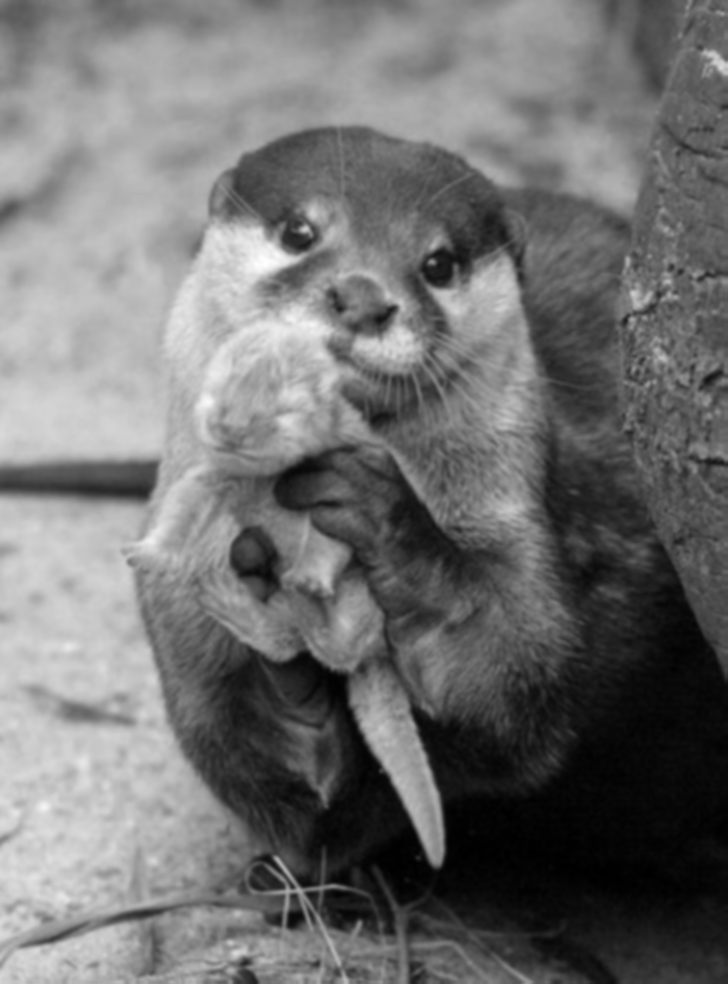
\includegraphics[width=0.95\linewidth]{gaussian_7.png}
        \caption{Размытие Гаусса, ядро 7x7}
    \end{subfigure}%%
    \begin{subfigure}[b]{0.5\linewidth}
        \centering
        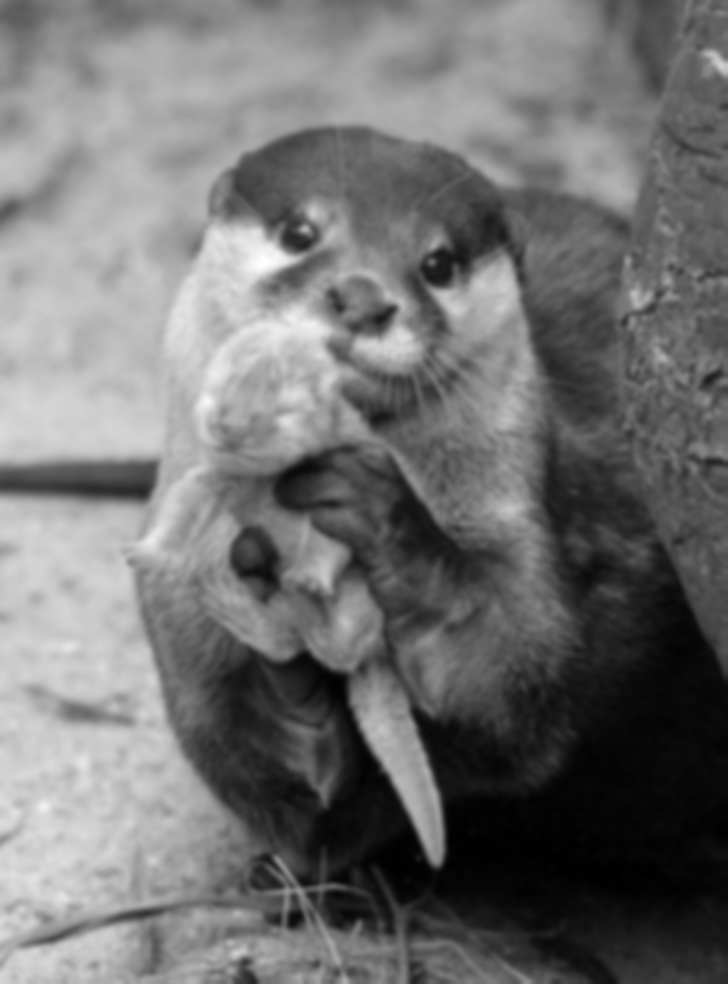
\includegraphics[width=0.95\linewidth]{gaussian_11.png}
        \caption{Размытие Гаусса, ядро 11x11}
    \end{subfigure}
    \caption{Размытие Гаусса (через теорему о свертке)}
    \label{img:gauss2}
\end{figure}

Видим, что результаты совпадают с результатами, полученными в предыдущем пункте. Таким образом, можно сделать вывод, 
что теорема о свертке работает корректно и в двумерном случае. 

Сравнивая результаты размытия Гаусса и блочного размытия, можно сделать вывод, что размытие Гаусса более плавное, чем блочное размытие.  Блочное размытие действует однообразно на все пиксели внутри ядра, в то время как размытие Гаусса учитывает расстояние от пикселя до центра ядра. 

\FloatBarrier
\section{Увеличение резкости}

Ядро для увеличения резкости изображения имеет вид:
\begin{equation}
    \begin{pmatrix}
        0 & -1 & 0 \\
        -1 & 5 & -1 \\
        0 & -1 & 0
    \end{pmatrix}
\end{equation}

Применим его к исходному изображению. Результат представлен на рисунке \ref{img:sharp}

\begin{figure}[ht!]
    \centering
    \begin{subfigure}[b]{0.5\linewidth}
        \centering
        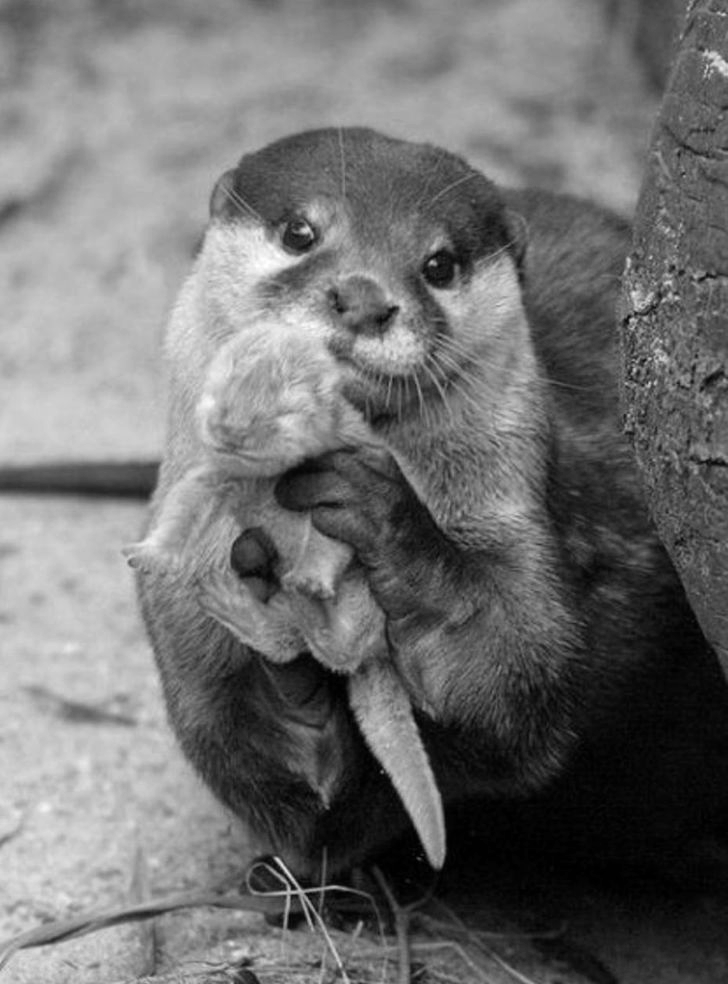
\includegraphics[width=0.95\linewidth]{bw.png}
        \caption{Исходное изображение}
    \end{subfigure}%%
    \begin{subfigure}[b]{0.5\linewidth}
        \centering
        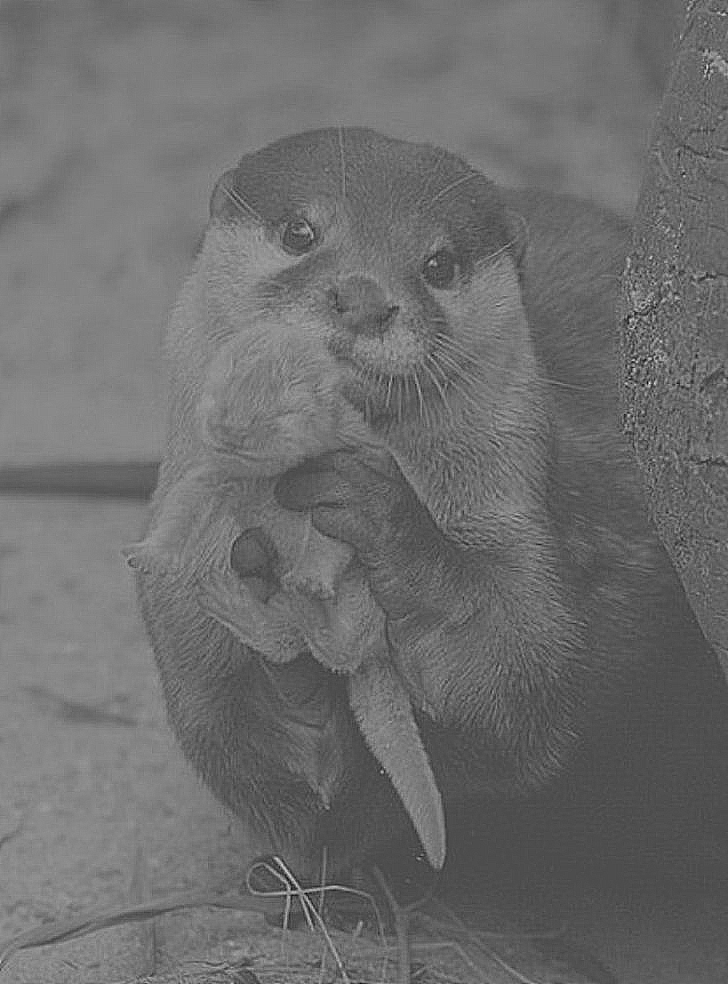
\includegraphics[width=0.95\linewidth]{laplacian.png}
        \caption{Увеличение резкости}
    \end{subfigure}
    \caption{Увеличение резкости}
    \label{img:sharp}
\end{figure}

Видим, что изображение стало более резким, чем было изначально, шерсть выдры стала более различимой. При этом изображение стало более темным. 

Результаты увеличения резкости с использованием теоремы о свертке представлены на рисунке \ref{img:sharp2}

\begin{figure}[ht!]
    \centering
    \begin{subfigure}[b]{0.5\linewidth}
        \centering
        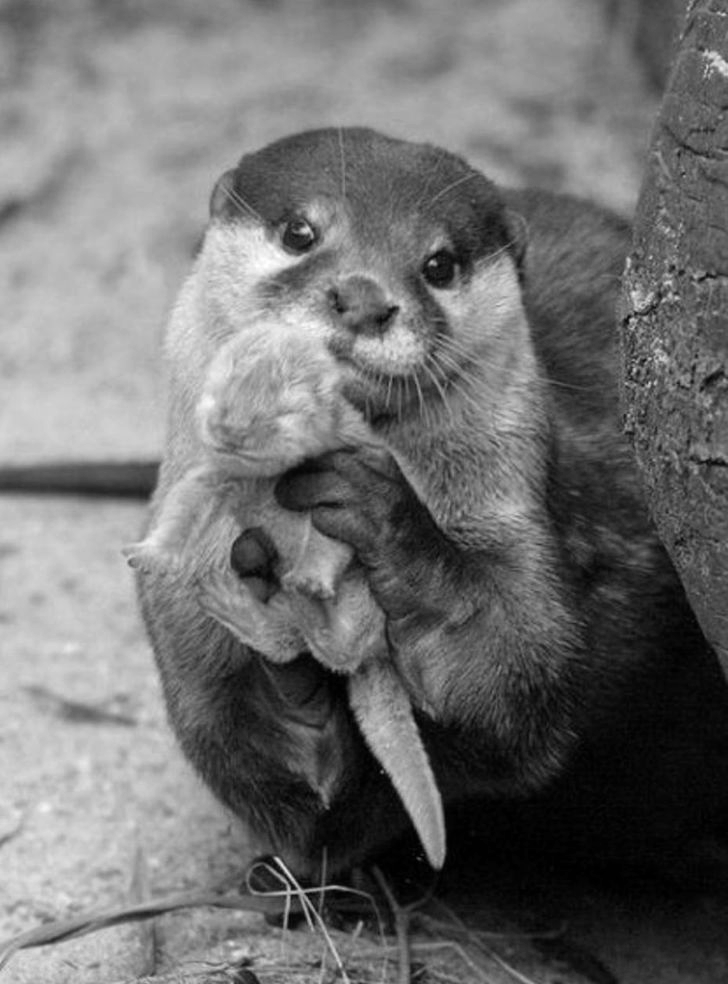
\includegraphics[width=0.95\linewidth]{bw.png}
        \caption{Исходное изображение}
    \end{subfigure}%%
    \begin{subfigure}[b]{0.5\linewidth}
        \centering
        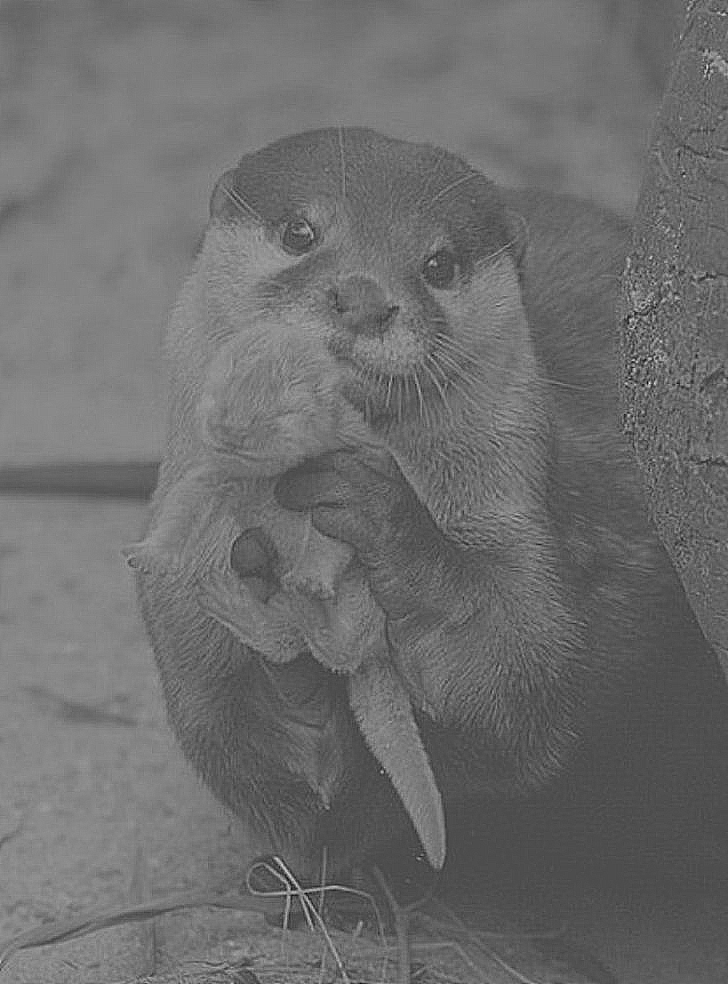
\includegraphics[width=0.95\linewidth]{laplacian.png}
        \caption{Увеличение резкости}
    \end{subfigure}
    \caption{Увеличение резкости (через теорему о свертке)}
    \label{img:sharp2}
\end{figure}

Результаты опять совпали, чего и следовало ожидать.

\FloatBarrier
\section{Выделение краев}

Ядро для выделения краев имеет вид:
\begin{equation}
    \begin{pmatrix}
        -1 & -1 & -1 \\
        -1 & 8 & -1 \\
        -1 & -1 & -1
    \end{pmatrix}
\end{equation}

Применим его к исходному изображению. Результат представлен на рисунке \ref{img:edge}

\begin{figure}[ht!]
    \centering
    \begin{subfigure}[b]{0.5\linewidth}
        \centering
        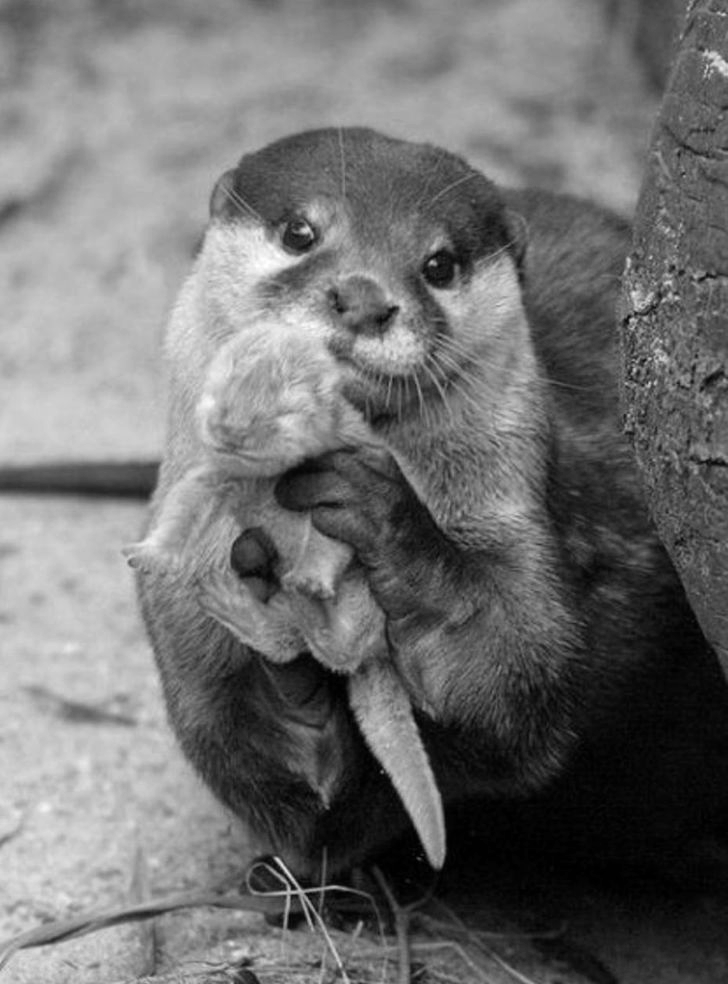
\includegraphics[width=0.95\linewidth]{bw.png}
        \caption{Исходное изображение}
    \end{subfigure}%%
    \begin{subfigure}[b]{0.5\linewidth}
        \centering
        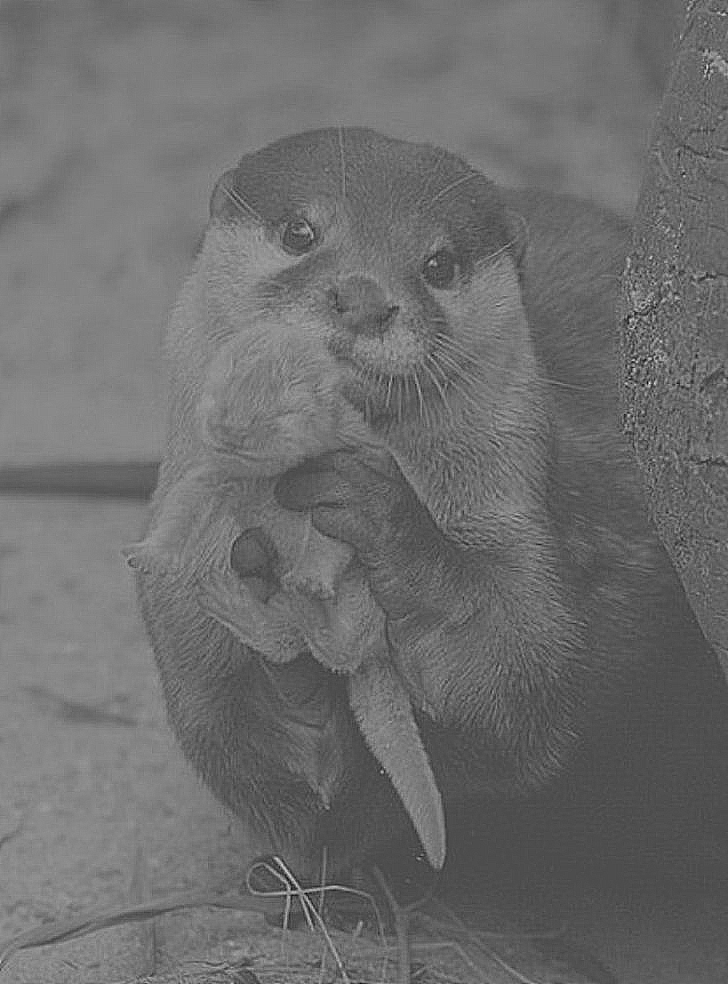
\includegraphics[width=0.95\linewidth]{edge_x.png}
        \caption{Выделение краев}
    \end{subfigure}
    \caption{Выделение краев}
    \label{img:edge}
\end{figure}

Видим, что изображение стало менее контрастным, но края объектов стали более выраженными.

Результаты выделения краев с использованием теоремы о свертке представлены на рисунке \ref{img:edge2}

\begin{figure}[ht!]
    \centering
    \begin{subfigure}[b]{0.5\linewidth}
        \centering
        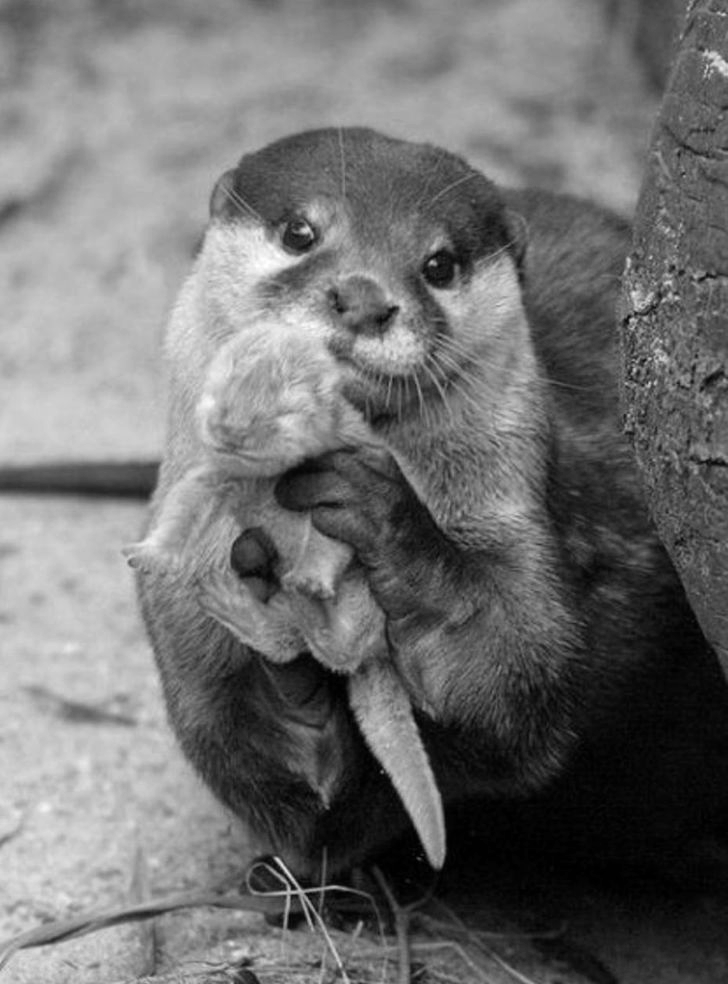
\includegraphics[width=0.95\linewidth]{bw.png}
        \caption{Исходное изображение}
    \end{subfigure}%%
    \begin{subfigure}[b]{0.5\linewidth}
        \centering
        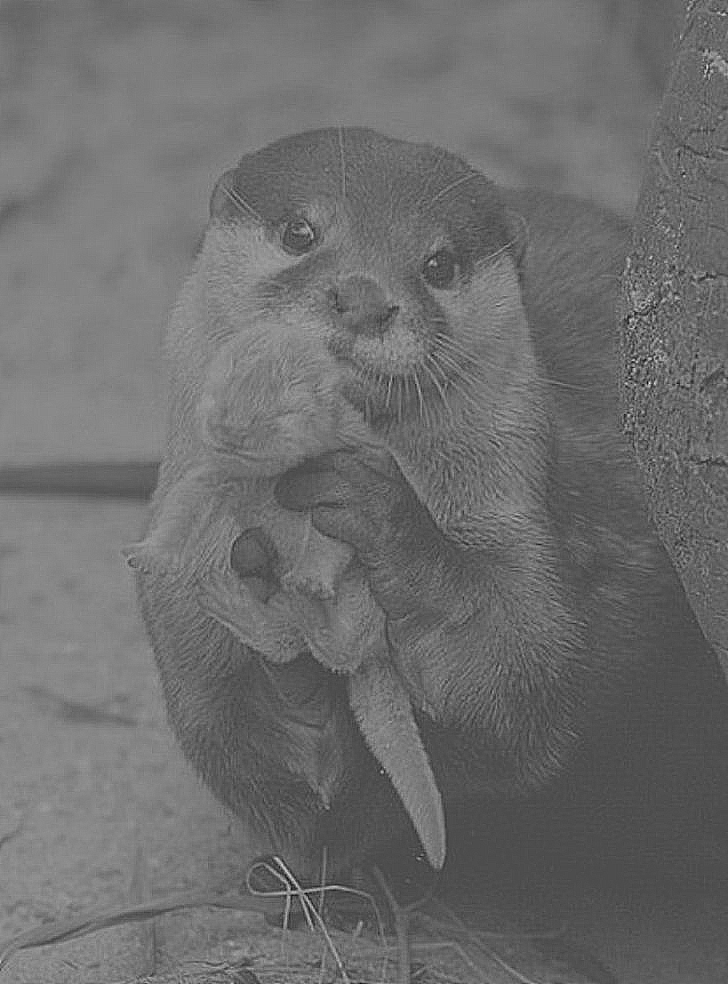
\includegraphics[width=0.95\linewidth]{edge_x.png}
        \caption{Выделение краев}
    \end{subfigure}
    \caption{Выделение краев (через теорему о свертке)}
    \label{img:edge2}
\end{figure}

Результаты опять совпали. Можно сделать вывод, что теорема о свертке работает корректно и в двумерном случае. 

\FloatBarrier